\chapter{System design}

\section{Architecture}


\begin{figure}[H]
	\centering
	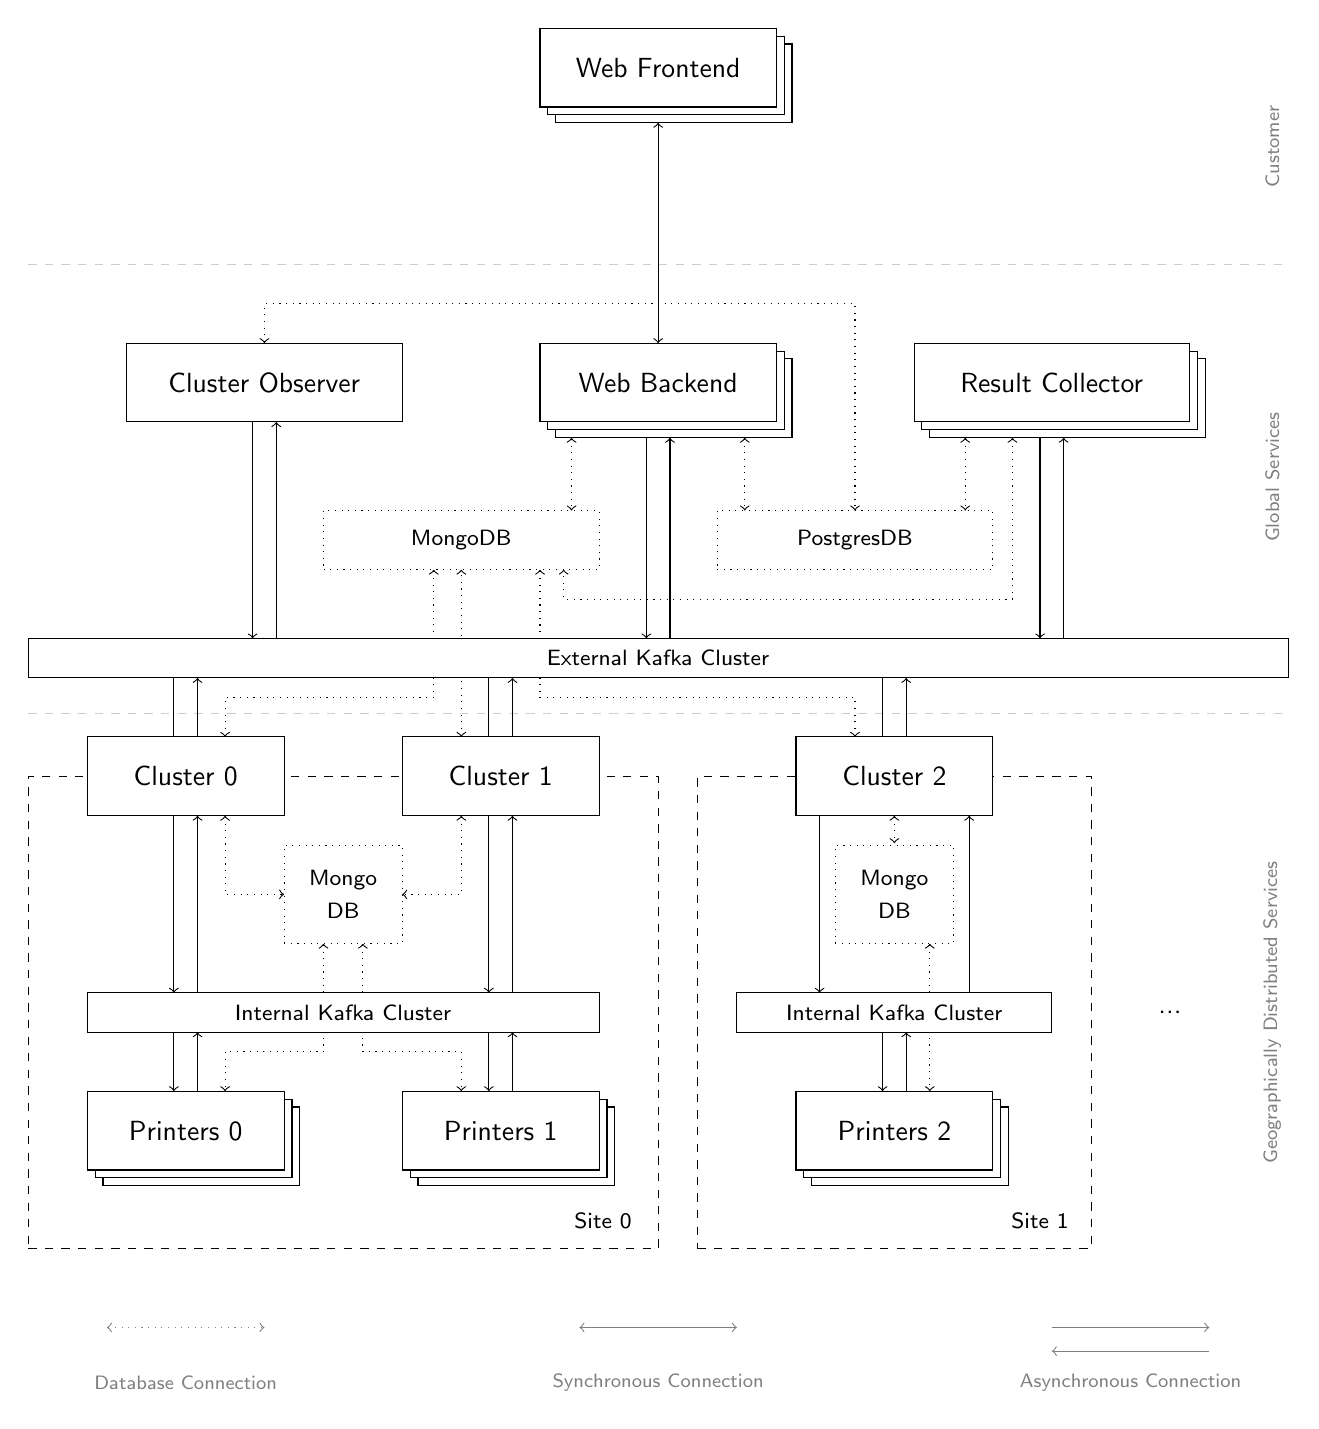
\begin{tikzpicture}
	
	\draw[-,dashed,draw=black!20!white] (-8cm, 1.5cm) to (8cm, 1.5cm);
	\draw[-,dashed,draw=black!20!white] (-8cm, -4.2cm) to (8cm, -4.2cm);
	
	\node[draw=black,fill=white,minimum width=3cm,align=center,minimum height=1cm] (frontend1) at (0.2cm, 3.8cm) {};
	\node[draw=black,fill=white,minimum width=3cm,align=center,minimum height=1cm] (frontend0) at (0.1cm, 3.9cm) {};
	\node[draw=black,fill=white,minimum width=3cm,align=center,minimum height=1cm] (frontend) at (0, 4) {\textsf{Web Frontend}};
	
	\draw[<->] (0cm, 3.3cm) to (0cm, 0.5cm);
	
	\node[draw=black,fill=white,minimum width=3cm,align=center,minimum height=1cm] (backend1) at (0.2cm, -0.2cm) {};
	\node[draw=black,fill=white,minimum width=3cm,align=center,minimum height=1cm] (backend0) at (0.1cm, -0.1cm) {};
	\node[draw=black,fill=white,minimum width=3cm,align=center,minimum height=1cm] (backend) at (0, 0) {\textsf{Web Backend}};
	
	\draw[->] (-0.15cm, -0.7cm) to (-0.15cm, -3.25cm);
	\draw[<-] (0.15cm, -0.7cm) to (0.15cm, -3.25cm);
	
	\node[draw=black,fill=white,minimum width=3.5cm,align=center,minimum height=1cm] (clusterObserver) at (-5, 0) {\textsf{Cluster Observer}};
	
	\draw[->] (-5.15cm, -0.5cm) to (-5.15cm, -3.25cm);
	\draw[<-] (-4.85cm, -0.5cm) to (-4.85cm, -3.25cm);
	
	\node[draw=black,fill=white,minimum width=3.5cm,align=center,minimum height=1cm] (resultCollector1) at (5.2cm, -0.2cm) {};
	\node[draw=black,fill=white,minimum width=3.5cm,align=center,minimum height=1cm] (resultCollector0) at (5.1cm, -0.1cm) {};
	\node[draw=black,fill=white,minimum width=3.5cm,align=center,minimum height=1cm] (resultCollector) at (5, 0) {\textsf{Result Collector}};
	
	\draw[->] (4.85cm, -0.7cm) to (4.85cm, -3.25cm);
	\draw[<-] (5.15cm, -0.7cm) to (5.15cm, -3.25cm);
	
	\draw[<->,dotted] (-5.5cm, -4.5cm) |- (-5.5cm, -4cm) -| (-2.85cm, -2.375cm);
	\draw[<->,dotted] (2.5cm, -4.5cm) |- (2.5cm, -4cm) -| (-1.5cm, -2.375cm);
	\draw[<->,dotted] (-2.5cm, -4.5cm) to (-2.5cm, -2.375cm);
	
	\draw[<->,dotted] (-1.1cm, -0.7cm) to (-1.1cm, -1.625cm);
	\draw[<->,dotted] (1.1cm, -0.7cm) to (1.1cm, -1.625cm);
	
	\draw[<->,dotted] (3.9cm, -0.7cm) to (3.9cm, -1.625cm);
	
	\draw[<->,dotted] (-5cm, 0.5cm) |- (-5cm, 1cm) to (2.5cm, 1cm) -| (2.5cm, -1.625cm);
	
	\draw[<->,dotted] (4.5cm, -0.7cm) |- (4.5cm, -2.75cm) to (-1.2cm, -2.75cm) -| (-1.2cm, -2.375cm);
	
	\node[draw=black,fill=white,minimum width=16cm,align=center,minimum height=0.5cm] (externalKafka) at (0cm, -3.5cm) {\footnotesize \textsf{External Kafka Cluster}};
	
	\node[draw=black,fill=white,minimum width=3.5cm,align=center,minimum height=0.75cm,dotted] (mongoDB) at (-2.5, -2) {\footnotesize \textsf{MongoDB}};
	
	\node[draw=black,fill=white,minimum width=3.5cm,align=center,minimum height=0.75cm,dotted] (postgresDB) at (2.5, -2) {\footnotesize \textsf{PostgresDB}};
	
	\node[draw=black,fill=white,minimum width=8cm,align=center,minimum height=6cm,dashed] (site0) at (-4, -8) {};
	
	\draw[<->,dotted] (-5.5cm, -5.5cm) |- (-4.75cm, -6.5cm);
	\draw[<->,dotted] (-2.5cm, -5.5cm) |- (-3.25cm, -6.5cm);
	
	\draw[<->,dotted] (-4.25cm, -7.125cm) |- (-5cm, -8.5cm) -| (-5.5cm, -9cm);
	\draw[<->,dotted] (-3.75cm, -7.125cm) |- (-3cm, -8.5cm) -| (-2.5cm, -9cm);
	
	\node[draw=black,fill=white,minimum width=6.5cm,align=center,minimum height=0.5cm] (kafka0) at (-4cm, -8cm) {\footnotesize \textsf{Internal Kafka Cluster}};
	
	\draw[->] (-6.15cm, -3.75cm) to (-6.15cm, -4.75cm);
	\draw[<-] (-5.85cm, -3.75cm) to (-5.85cm, -4.75cm);
	
	\node[draw=black,fill=white,minimum width=2.5cm,align=center,minimum height=1cm] (cluster0) at (-6, -5) {\textsf{Cluster 0}};
	
	\draw[->] (-6.15cm, -5.5cm) to (-6.15cm, -7.75cm);
	\draw[<-] (-5.85cm, -5.5cm) to (-5.85cm, -7.75cm);
	
	\draw[->] (-6.15cm, -8.25cm) to (-6.15cm, -9cm);
	\draw[<-] (-5.85cm, -8.25cm) to (-5.85cm, -9cm);
	
	\node[draw=black,fill=white,minimum width=1.5cm,align=center,minimum height=1.25cm,dotted] (mongoDB0) at (-4, -6.5) {\footnotesize \textsf{Mongo} \\ \footnotesize \textsf{DB}};
	
	\node[draw=black,fill=white,minimum width=2.5cm,align=center,minimum height=1cm] (printers00) at (-5.8, -9.7) {};	
	\node[draw=black,fill=white,minimum width=2.5cm,align=center,minimum height=1cm] (printers01) at (-5.9, -9.6) {};	
	\node[draw=black,fill=white,minimum width=2.5cm,align=center,minimum height=1cm] (printers0) at (-6, -9.5) {\textsf{Printers 0}};
	
	\draw[->] (-2.15cm, -3.75cm) to (-2.15cm, -4.75cm);
	\draw[<-] (-1.85cm, -3.75cm) to (-1.85cm, -4.75cm);
	
	\node[draw=black,fill=white,minimum width=2.5cm,align=center,minimum height=1cm] (cluster1) at (-2, -5) {\textsf{Cluster 1}};
	
	\draw[->] (-2.15cm, -5.5cm) to (-2.15cm, -7.75cm);
	\draw[<-] (-1.85cm, -5.5cm) to (-1.85cm, -7.75cm);
	
	\draw[->] (-2.15cm, -8.25cm) to (-2.15cm, -9cm);
	\draw[<-] (-1.85cm, -8.25cm) to (-1.85cm, -9cm);
	
	\node[draw=black,fill=white,minimum width=2.5cm,align=center,minimum height=1cm] (printers10) at (-1.8, -9.7) {};	
	\node[draw=black,fill=white,minimum width=2.5cm,align=center,minimum height=1cm] (printers10) at (-1.9, -9.6) {};	
	\node[draw=black,fill=white,minimum width=2.5cm,align=center,minimum height=1cm] (printers1) at (-2, -9.5) {\textsf{Printers 1}};
	
	\node[draw=black,fill=white,minimum width=5cm,align=center,minimum height=6cm,dashed] (site1) at (3, -8) {};
	
	\draw[<->,dotted] (3.45cm, -7.125cm) to (3.45cm, -9cm);
	
	\draw[<->,dotted] (3cm, -5.5cm) to (3cm, -5.85cm);
	
	\node[draw=black,fill=white,minimum width=4cm,align=center,minimum height=0.5cm] (kafka1) at (3cm, -8cm) {\footnotesize \textsf{Internal Kafka Cluster}};
	
	\draw[->] (2.85cm, -3.75cm) to (2.85cm, -4.75cm);
	\draw[<-] (3.15cm, -3.75cm) to (3.15cm, -4.75cm);
	
	\node[draw=black,fill=white,minimum width=2.5cm,align=center,minimum height=1cm] (cluster2) at (3, -5) {\textsf{Cluster 2}};
	
	\draw[->] (2.05cm, -5.5cm) to (2.05cm, -7.75cm);
	\draw[<-] (3.95cm, -5.5cm) to (3.95cm, -7.75cm);
	
	\node[draw=black,fill=white,minimum width=1.5cm,align=center,minimum height=1.25cm,dotted] (mongoDB0) at (3, -6.5) {\footnotesize \textsf{Mongo} \\ \footnotesize \textsf{DB}};
	
	\draw[->] (2.85cm, -8.25cm) to (2.85cm, -9cm);
	\draw[<-] (3.15cm, -8.25cm) to (3.15cm, -9cm);
	
	\node[draw=black,fill=white,minimum width=2.5cm,align=center,minimum height=1cm] (printers20) at (3.2, -9.7) {};	
	\node[draw=black,fill=white,minimum width=2.5cm,align=center,minimum height=1cm] (printers20) at (3.1, -9.6) {};	
	\node[draw=black,fill=white,minimum width=2.5cm,align=center,minimum height=1cm] (printers2) at (3, -9.5) {\textsf{Printers 2}};
	
	\node[draw=white,fill=white,align=center] (dots) at (6.5, -8) {\textsf{...}};
	
	\node[draw=white,fill=white,align=center,text=gray,rotate=90] (distributedServices) at (7.8, -8) {\scriptsize \textsf{Geographically Distributed Services}};
	
	\node[draw=white,fill=white,align=center,text=gray,rotate=90] (centralServices) at (7.8, -1.2) {\scriptsize \textsf{Global Services}};
	
	\node[draw=white,fill=white,align=center,text=gray,rotate=90] (customer) at (7.8, 3) {\scriptsize \textsf{Customer}};
	
	\node[draw=white,fill=white,align=center] (labelSite0) at (-0.7, -10.65) {\footnotesize \textsf{Site 0}};
	\node[draw=white,fill=white,align=center] (labelSite0) at (4.85, -10.65) {\footnotesize \textsf{Site 1}};	
	
	\draw[<->,dotted,draw=gray] (-7cm, -12cm) to (-5cm, -12cm);
	\node[draw=white,fill=white,align=center,text=gray] (databaseConnection) at (-6, -12.7) {\scriptsize \textsf{Database Connection}};
	
	
	\draw[<->,draw=gray] (-1cm, -12cm) to (1cm, -12cm);
	\node[draw=white,fill=white,align=center,text=gray] (databaseConnection) at (0, -12.7) {\scriptsize \textsf{Synchronous Connection}};
	
	\draw[->,draw=gray] (5cm, -12cm) to (7cm, -12cm);
	\draw[<-,draw=gray] (5cm, -12.3cm) to (7cm, -12.3cm);
	\node[draw=white,fill=white,align=center,text=gray] (databaseConnection) at (6, -12.7) {\scriptsize \textsf{Asynchronous Connection}};
	
	\end{tikzpicture}
	\caption{System Concept Overview}
	\label{system:concept}
\end{figure}


event based

common file system for communication because minimum requirements

stick to unix principles(list): simple, human readable intermediate format

voting/election by capabilities and 'will' of a node to run a stage

\section{Communication/Event architecture?}

\section{Targeting capabilities}

\subsection{General thoughts}

\section{Planned}

\section{Implementation details}

\section{Synchronization, Locking, publishing events}

\section{REST for UI}



\section{Event Bus}

requires common a way to exchange messages

all messages - called events - are published to all nodes

using file system as bus

clear and globally same order of events

events consist of an id, command, time, duration, subject and issuer

events might have a duration

unspoken requirement: all nodes share the same clock - or one with very little drift

\subsection{Atomicy of (Unix) Filesystems}

\subsection{Atomicy and behavior of NFS in particular}

\subsection{Using as lock backend}

\subsection{Using as election backend}



\section{Election System}

Utilizing Event Bus for timely limited elections and to ensure that there are no concurrent election for a single project.

\todo{what about concurrent elections on multiple projects}